\section{Konfigurationer af højtalerkabinettet}
I dette afsnit vil der blive set på hvordan forskellige konfigurationer af højtalerkabinettet påvirker dets frekvenskarakteristik. Idet det udelukkende er kabinettets egen karakteristik der er interessant i denne sammenhæng, så er det altså ikke ønskeligt, at rummets udformning spiller nogen større rolle i den samlede frekvenskarakteristik.

For at minimere rummets betydning for den samlede frekvenskarakteristik så blev højtaleren placeret i det lyddøde rum på IHA. Herved blev eventuelle reflektioner (ekkoer) dæmpet og det samme blev deres indvirkning på det samlede frekvensrespons.
\begin{figure}[H]
	\centering
	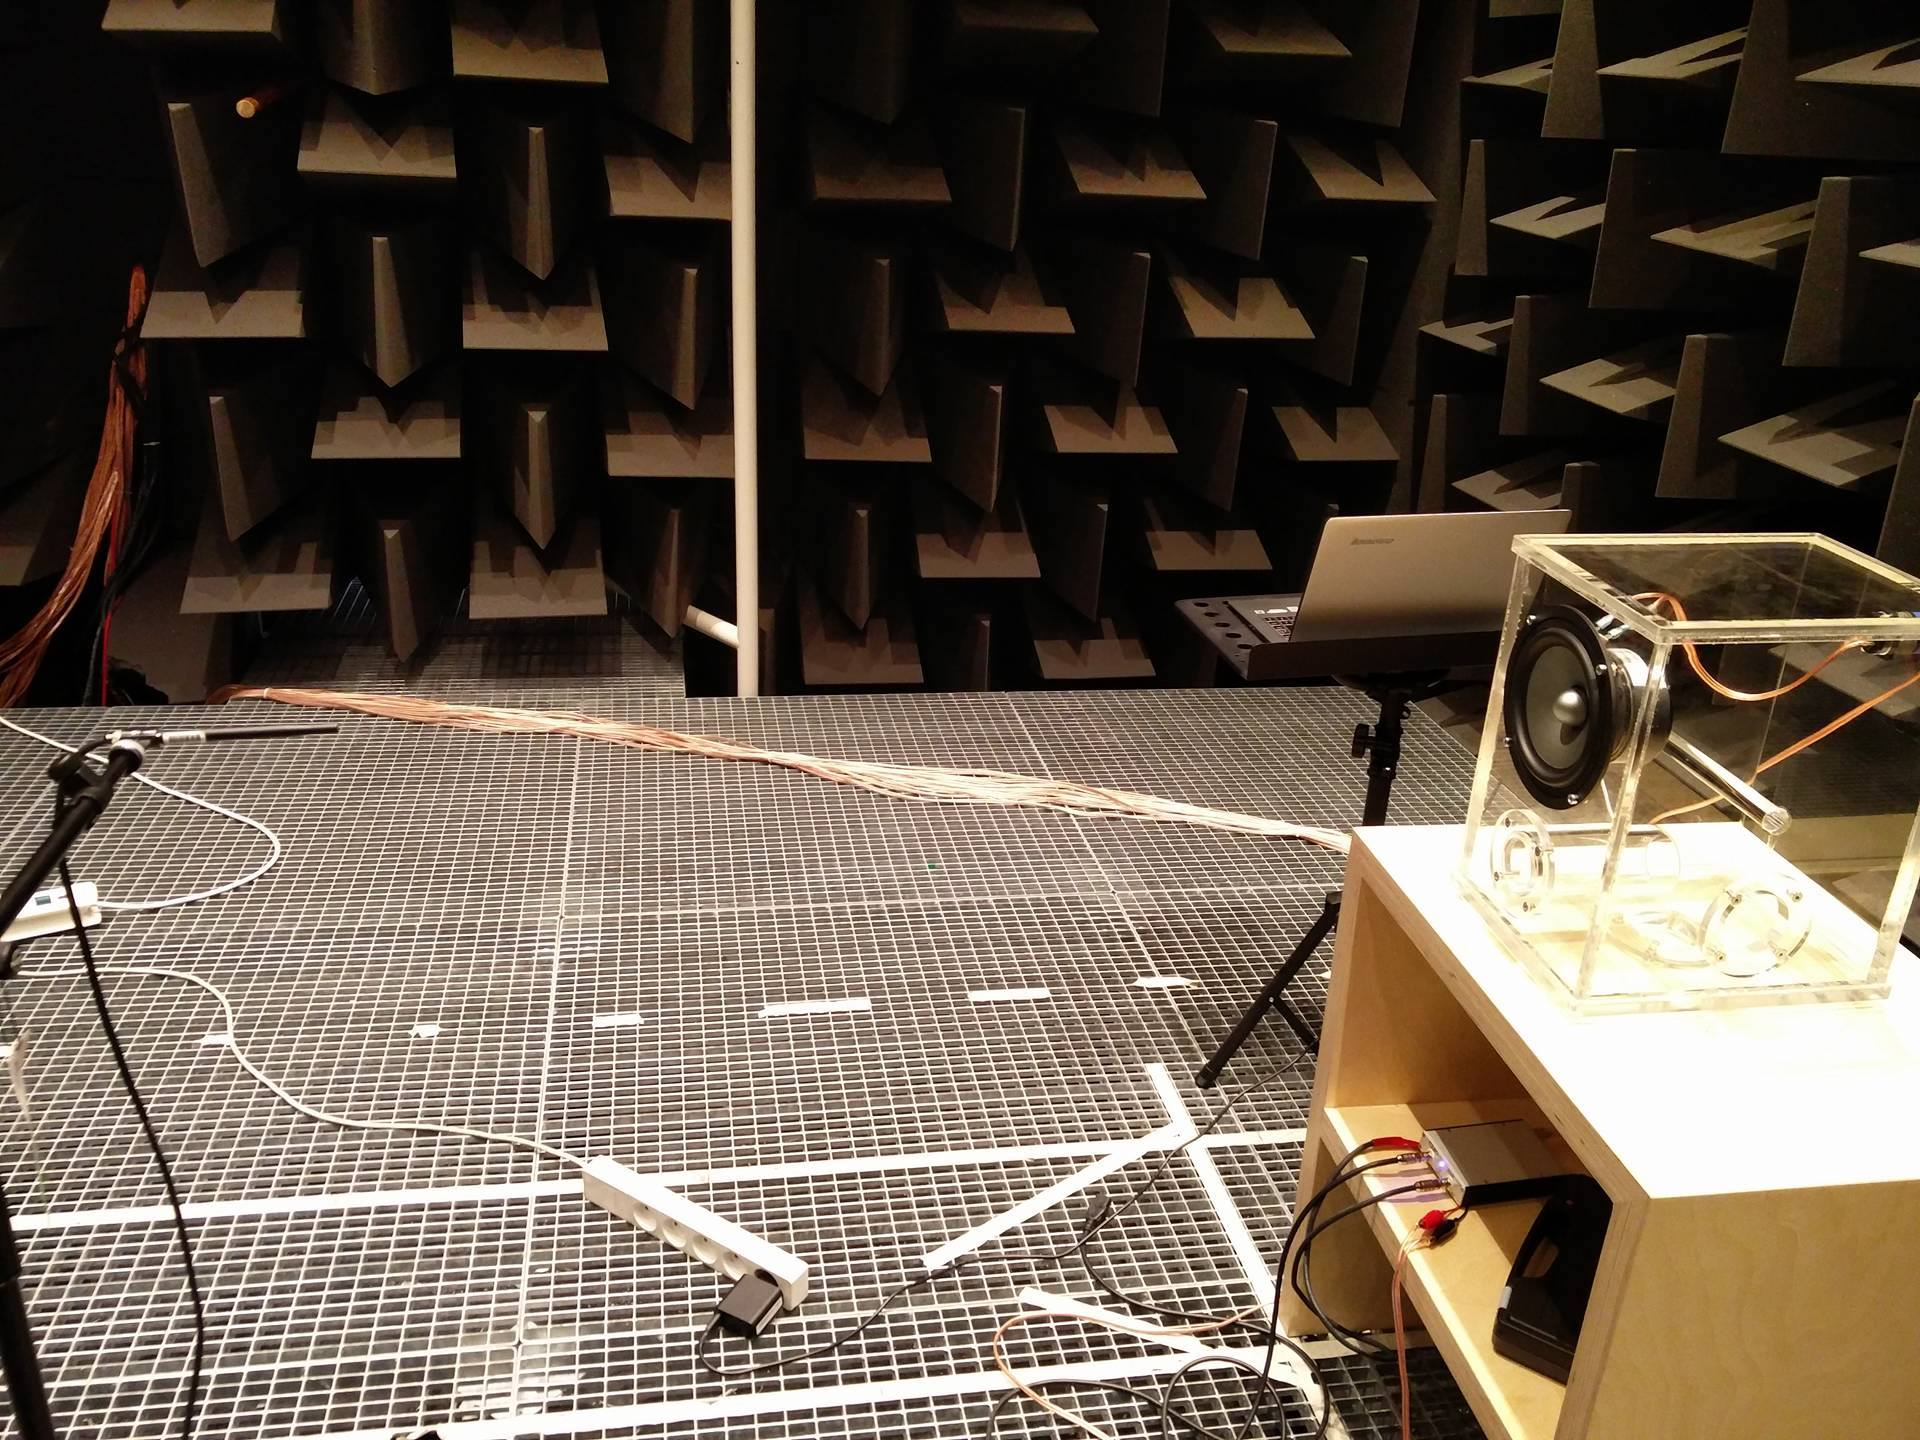
\includegraphics[width=0.8\textwidth]{Billeder/LyddodtRum}
	\caption{Typisk måleopstilling i det lyddøde rum}
\end{figure}

Højtalerkabinettet er lavet til, at kunne konfigureres med forskellige længder basrefleksrør som kan placeres forskellige steder. De forskellige rørlængder der er blevet undersøgt i denne report er: \SI{3,5}{\centi\meter}, \SI{7,0}{\centi\meter} og \SI{15,0}{\centi\meter}. De vil efterfølgende, meget naturligt, blive referet til som Kort, Medium og Lang basrefleks.

Basreflekserne kan som sagt placeres forskellige steder på højtalerkabinettet: Foran under membranen, på siden i samme højde som basrefleksen foran og under bunden. De vil på de efterfølgende sider blive refereret til som Forside, Side og Bund.

I undersøgelserne vil der kun blive placeret et basrefleksrør i kabinettet ad gangen og alle andre huller vil blive forseglet med en lufttæt prop. Disse propper kan også bruges til, at lave et helt forseglet kabinet - som også vil blive undersøgt på de følgende sider.

\newpage
\subsection{Lukket kabinet}
Der blev først og fremmest set på karakteristikken for et helt lukket kabinet. Det vil altså sige, at alle propper blev sat over basreflekshullerne. Frekvenskarakteristikken blev herefter målt med CLIO Pocket lige foran membranen og i \SI{1}{\meter} afstand foran membranen. Resultatet af disse målinger ses på figuren nedenfor.\fixme{inkluder simulering i figuren. Derudover ville lidt teori om frekvenskarakteristikken for et lukket kabinet være lækkert, inden vi kaster os ud i målinger. Også så vi kan sammenholde teori med praksis -AB}
\begin{figure}[H]
	\centering
	\vspace{-12pt}
	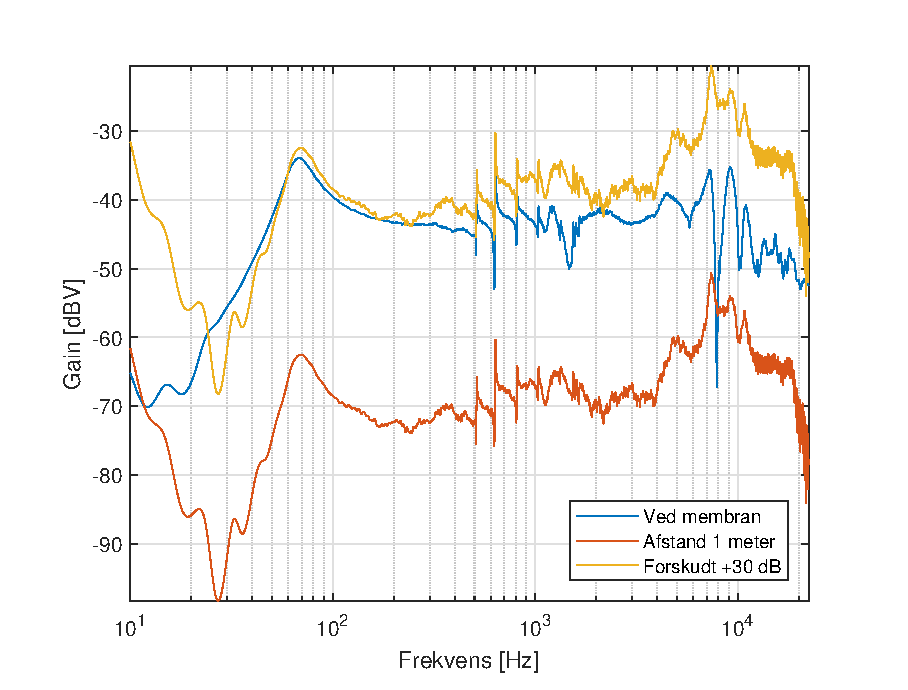
\includegraphics[width=\textwidth]{Billeder/Grafer/ClosedCabinet}
	\caption{Målinger på et lukket kabinet}
\end{figure}

Disse måleresultater udtaler sig som sagt ikke om hvordan basrefleksen påvirker frekvenskarakteristikken - men de vil blive brugt som referencemålinger i mange af de følgende måleopstillinger og resultater.

\begin{wrapfigure}{r}{0.5\textwidth} 
	\vspace{-20pt}
	\begin{center}
		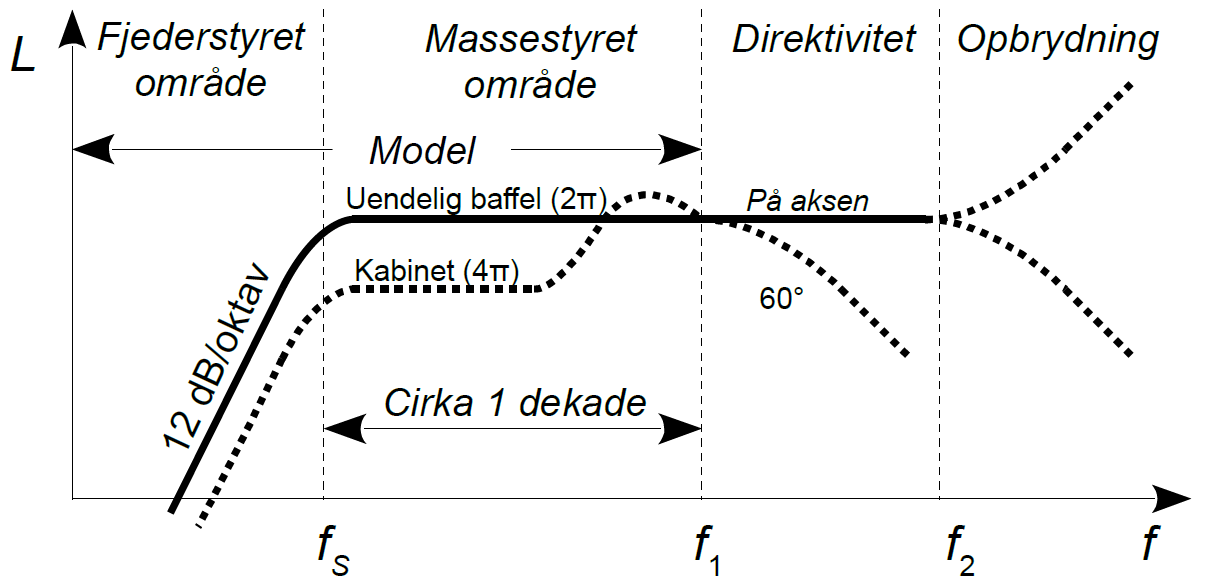
\includegraphics[width=0.5\textwidth]{Billeder/FrekvenskarakteristikTeori}
	\end{center}
	\vspace{-15pt}
	\caption{Teoretisk frekvenskarakteristik}
	\vspace{-20pt}
\end{wrapfigure}
På figuren ovenfor optræder nogenlunde den type karakteristik vi forventer. Det er især resonansfrekvensen $f_s$ ved \SI{70}{\hertz} som er meget interessant idet denne frekvens adskiller det \textbf{fjederstyrede område} fra det \textbf{massestyrede område}. Derudover er der blevet målt en hældning på kurven svarende til omkring +18 dB/oktav i det fjederstyrede område - altså en smule mere end den teoretiske stigning.

Hvis det, som omtalt i teorien, også antages at frekvensen $f_1$ ligger en dekade over $f_s$, så svarer denne frekvens altså til \SI{700}{\hertz}. Herefter vil direktiviteten begynde at spille en stor rolle på frekvenskarakteristikken.

På grafen ses det også, at når CLIO-mikrofonen flyttes længere væk fra membranen, så bevarer karakteristikken nogenlunde sin form i det massestyrede område og et godt stykke ind i både området over og under i frekvensspektret. Den største forskel er dog, at karakteristikken er blevet dæmpet med omkring -30 dB. Derfor er den ovenstående kurve målt i 1 meters afstand også blevet korrigeret med +30 dB for at vise dette. \fixme{Vi behøver vel ikke korrigere? Vi skal bare holde 1m afstand-måling sammen med 1m afstand, og tæt afstand med tæt afstand}

For at eftervise at dette er korrekt, så ses der på den nedenstående formel der giver en sammenhæng mellem lydtryk og afstand fra lydgiveren:
\begin{equation}
L_2 = L_1 - \left| 20 \cdot \log \left( \frac{r_1}{r_2} \right) \right|
\end{equation}

Hvor værdierne $L_1$ og $L_2$ er lydtryksniveauet målt i afstandene $r_1$ og $r_2$. Hvis der ses peaken omkring den første resonansfrekvens $f_s$, så ligger denne ved omkring $-\SI{34}{\decibel}$ når der måles tæt på højtaleren og $-\SI{62.5}{\decibel}$, når der måles i 1 meters afstand. Hvis disse værdier indsættes i den førnævnte formel, så findes der følgende:
\begin{equation}
\SI{-62.5}{\decibel} = \SI{-34}{\decibel} - \left| 20 \cdot \log \left( \frac{r_1}{\SI{1.00}{\meter}} \right)\right| \quad \Rightarrow \quad r_1 \approxeq \SI{3}{\centi\meter}
\end{equation}

Hvilket altså vil sige, at CLIO-mikrofonen har været placeret omkring \SI{3}{\centi\meter} fra højtaleren. Dette virker også meget sandsynligt.

Grunden til afvigelsen i det fjederstyrede område\fixme{ift hvad? - AB} kan skyldes, at dæmpningsfaktoren i luft er meget anderledes ved lave frekvenser\fixme{ref? - AB}. Afvigelsen ved de højere frekvenser skyldes at direktiviten spiller ind. Det kan derfor sagtens tænkes, at CLIO-mikrofonen ikke har stået præcist vinkelret ind på højtalerens midte. \fixme{Men netop de lavere frekvenser burde vel være ligeglade, da der her ikke spiller direktivitet ind (fjederstyret område) - AB}
\newpage
\subsection{Indflydelse af basrefleksens længde}
I dette afsnit vil der blive set på, hvordan længden af basrefleksen kommer til, at spille en rolle i kabinettets samlede frekvenskarakteristik. For at holde variabel-kontrol, så bliver der i første omgang kun målt på betydningen af længden, når basrefleksen er placeret på forsiden af kabinettet.

Der ønskes målt på to dele af højtalerkabinettet: Membranen og basrefleksrøret. Dette gøres ved, at placere CLIO-mikrofonen helt op ad membranen eller helt inde i basrefleksrøret. De to målinger kommer måske ikke til, at være helt akustiske adskilte, men dette er en fejlkilde man er nødt til at leve med.

I første omgang måles der kun på selve membranen, når basrefleksen sidder på forsiden. Resultaterne af disse målinger bliver opvejet med de målinger som blev fundet når kabinettet var helt lukket (ingen basrefleks). Resultatet af dette ses nedenfor.
\begin{figure}[H]
	\centering
	\vspace{-12pt}
	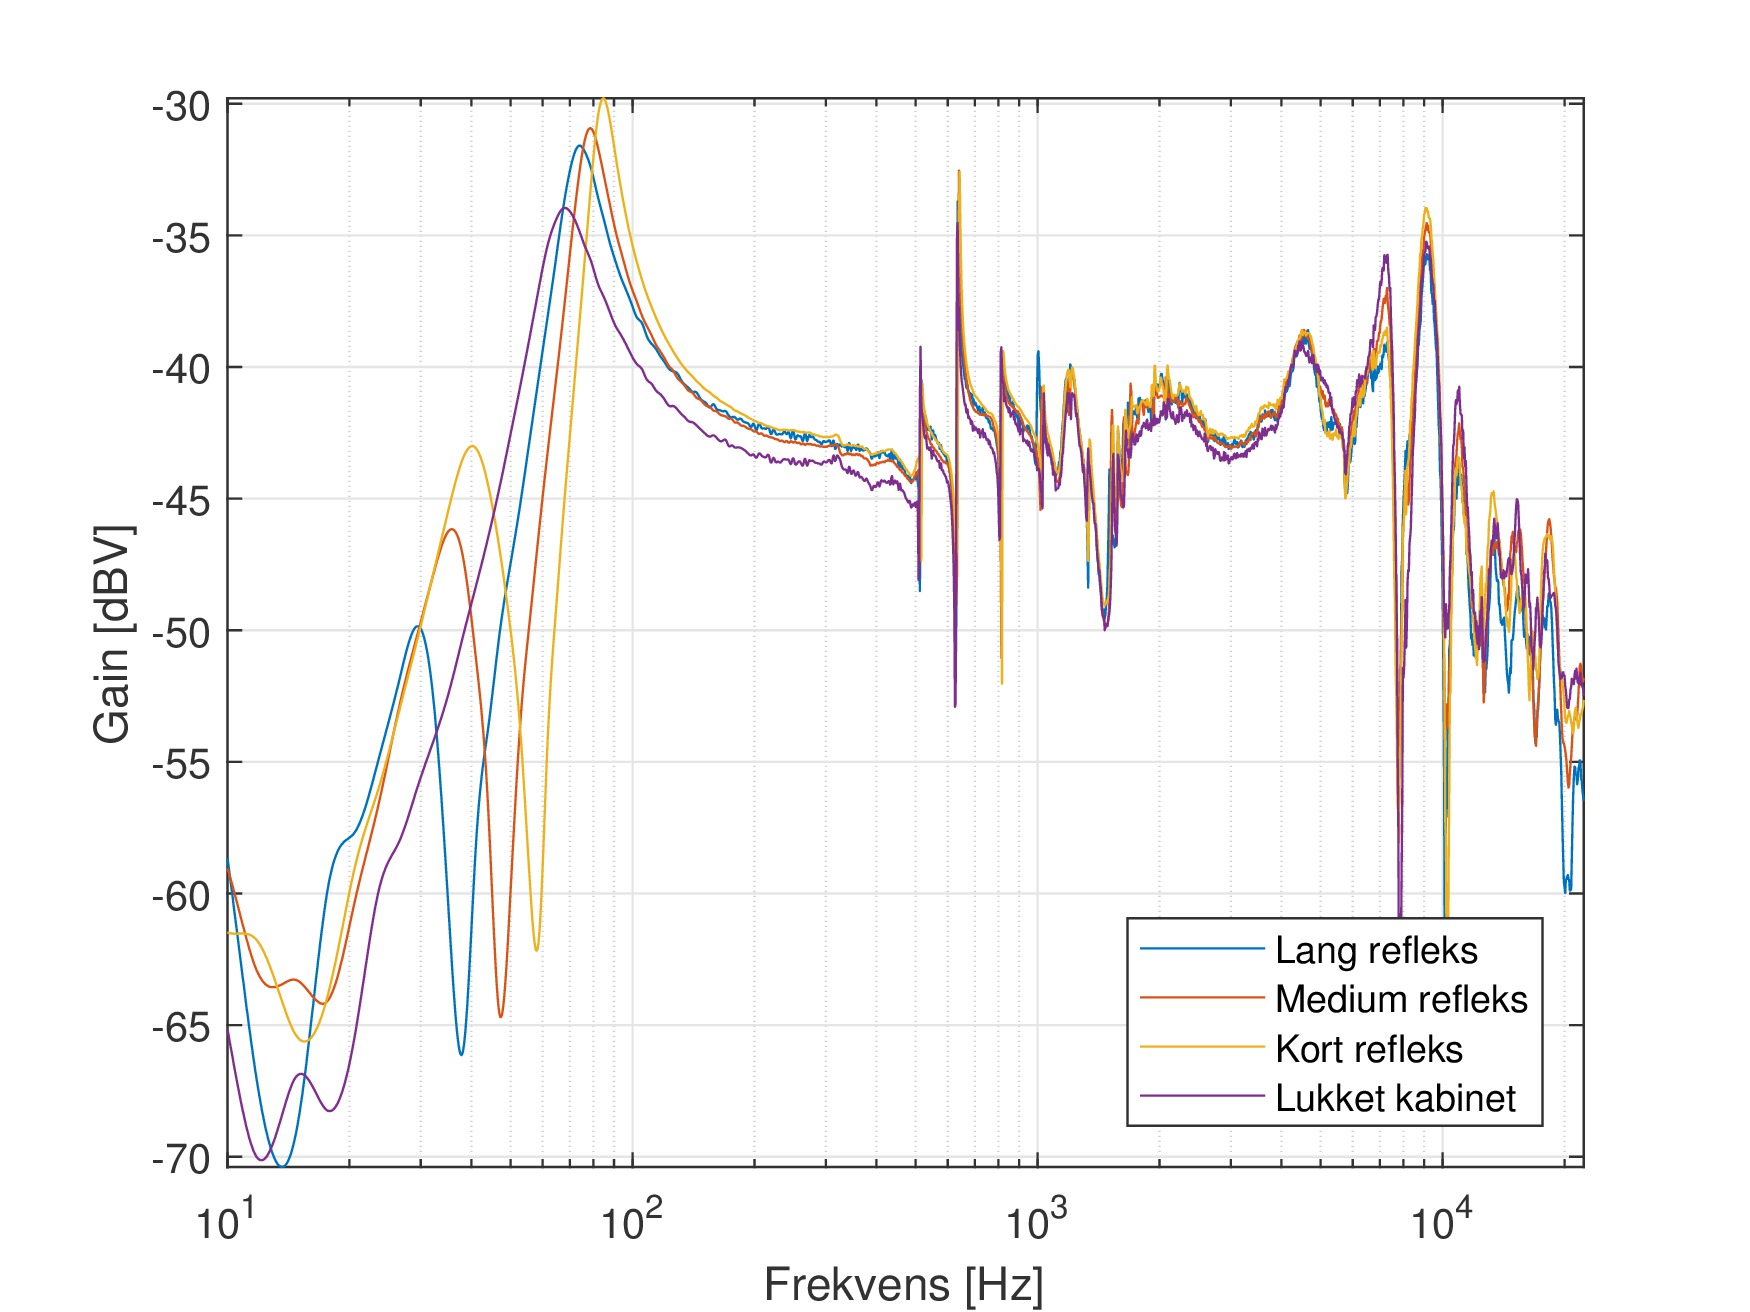
\includegraphics[width=\textwidth]{Billeder/Grafer/BasrefleksLengthMembran}
	\caption{Betydning af basrefleksens længde (målt på membran)}
\end{figure}

Det centrale ved de ovenstående måleresultater er, at der nu forekommer et 'forstærkningsdyk' omkring de lave frekvenser. Samtidig ændres både resonansfrekvensen $f_s$ placering og forstærkningen ved resonansfrekvensen, når der tilføjes en basrefleks eller ændres på længden af basrefleksen.

Det ses på figuren, at jo kortere basrefleksen bliver, jo højere op i både frekvens og forstærkning kommer resonansfrekvensen $f_s$. Samtidig ses det også, at jo længere basrefleksen bliver, jo længere ned i frekvens kommer forstærkningsdykket til at ligge, men at forstærkningen under denne faktisk stiger.

Næste skridt er, at se på selve basrefleksrørets frekvensrespons. Dette respons blev som sagt målt ved, at placere CLIO-mikrofonen inde i selve røret. Af gode grunde, så kan de målte resultater for basrefleksrøret ikke sammenlignes med målte data fra et lukket kabinet.
\begin{figure}[H]
	\centering
	\vspace{-12pt}
	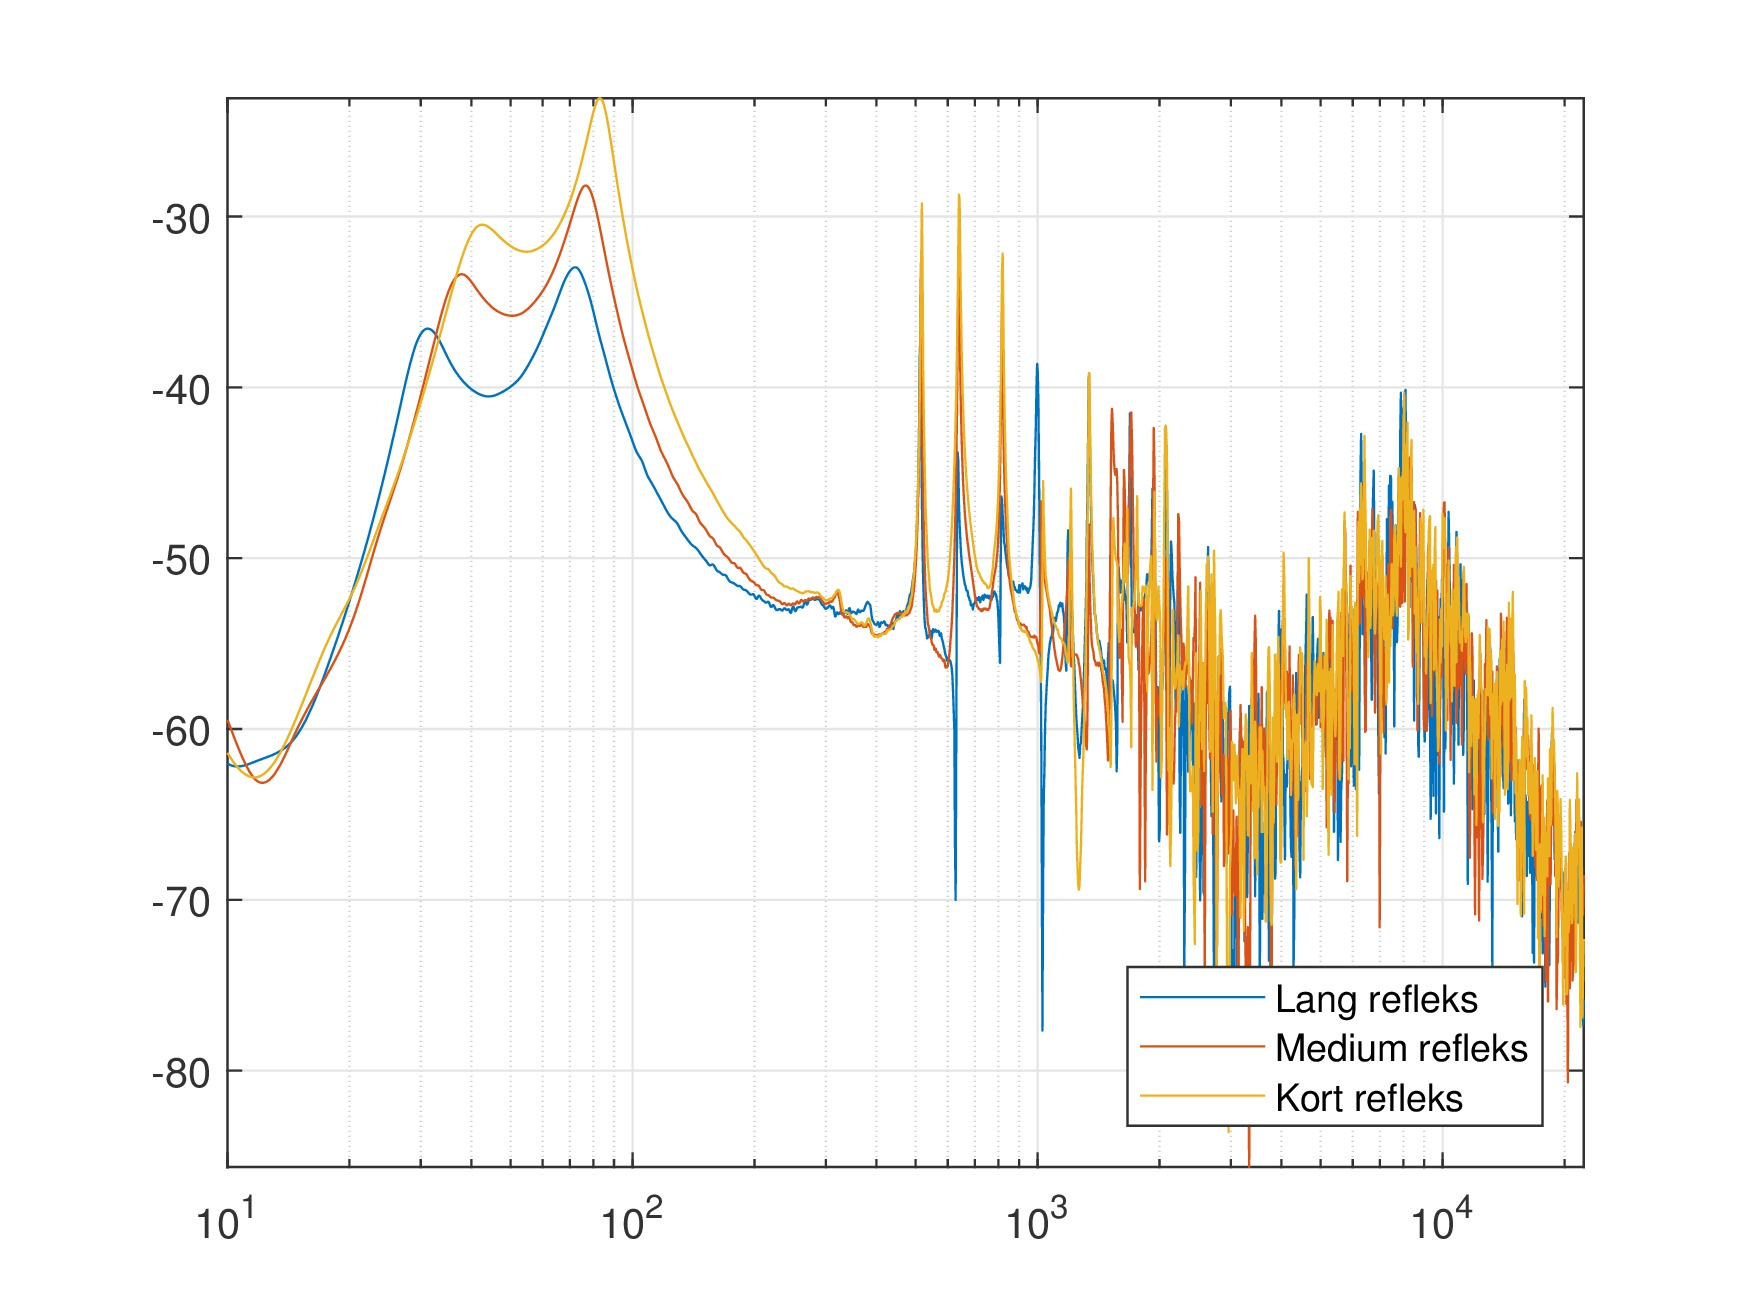
\includegraphics[width=\textwidth]{Billeder/Grafer/BasrefleksLengthTube}
	\caption{Betydning af basrefleksens længde (målt på basrefleks)}
\end{figure}

Den ovenstående figur vil kun blive undersøgt i frekvensområdet fra \SI{10}{\hertz} til \SI{300}{\hertz} idet det er her der ønskes en undersøgelse af basrefleksens indvirkning. Det ses at der optræder to peaks omkring noget der ligner en klassisk båndpaskarakteristik.

Når basrefleksen gøres kortere, så kommer de to peaks til, at give en større forstærkning, men kommer samtidig til, at ligge ved højere frekvenser. Hvis man ønsker en basrefleks der skal give kabinettet et 'løft' ved lave frekvenser, så skal man for dette højtalerkabinet med en lang basrefleks - altså \SI{15}{\centi\meter}.

\newpage
Til sidst blev der set på hvordan en lytter vil opleve lyden fra højtalerkabinettet. Dette blev gjort ved, at placere CLIO-mikrofonen i en afstand på \SI{1}{\meter} fra højtaleren. I dette område burde frekvenskarakteristikken fra membranen og karakteristikken fra basrefleksen ikke længere kunne skelnes, men bør i stedet opveje hinanden.
\begin{figure}[H]
	\centering
	\vspace{-12pt}
	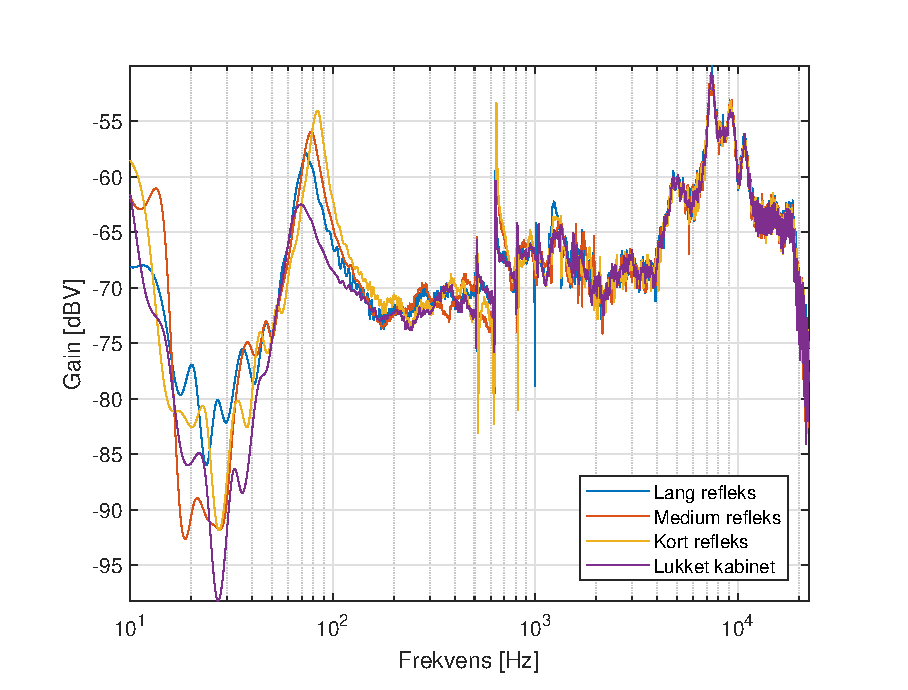
\includegraphics[width=\textwidth]{Billeder/Grafer/BasrefleksLengthFar}
	\caption{Betydning af basrefleksens længde (målt i lytteafstand)}
\end{figure}

Det ses, at ved at indsætte et basrefleksrør med længden \SI{15}{\centi\meter}, så stiger forstærkningen ved resonansfrekvensen med omkring \SI{7}{\decibel}. Derudover, så bliver forstærkningen ved de endnu lavere frekvenser (\SI{20}{\hertz} til \SI{40}{\hertz}) også højere med helt op til \SI{15}{\decibel} når der indsættes en lang basrefleks.
\begin{figure}[H]
	\centering
	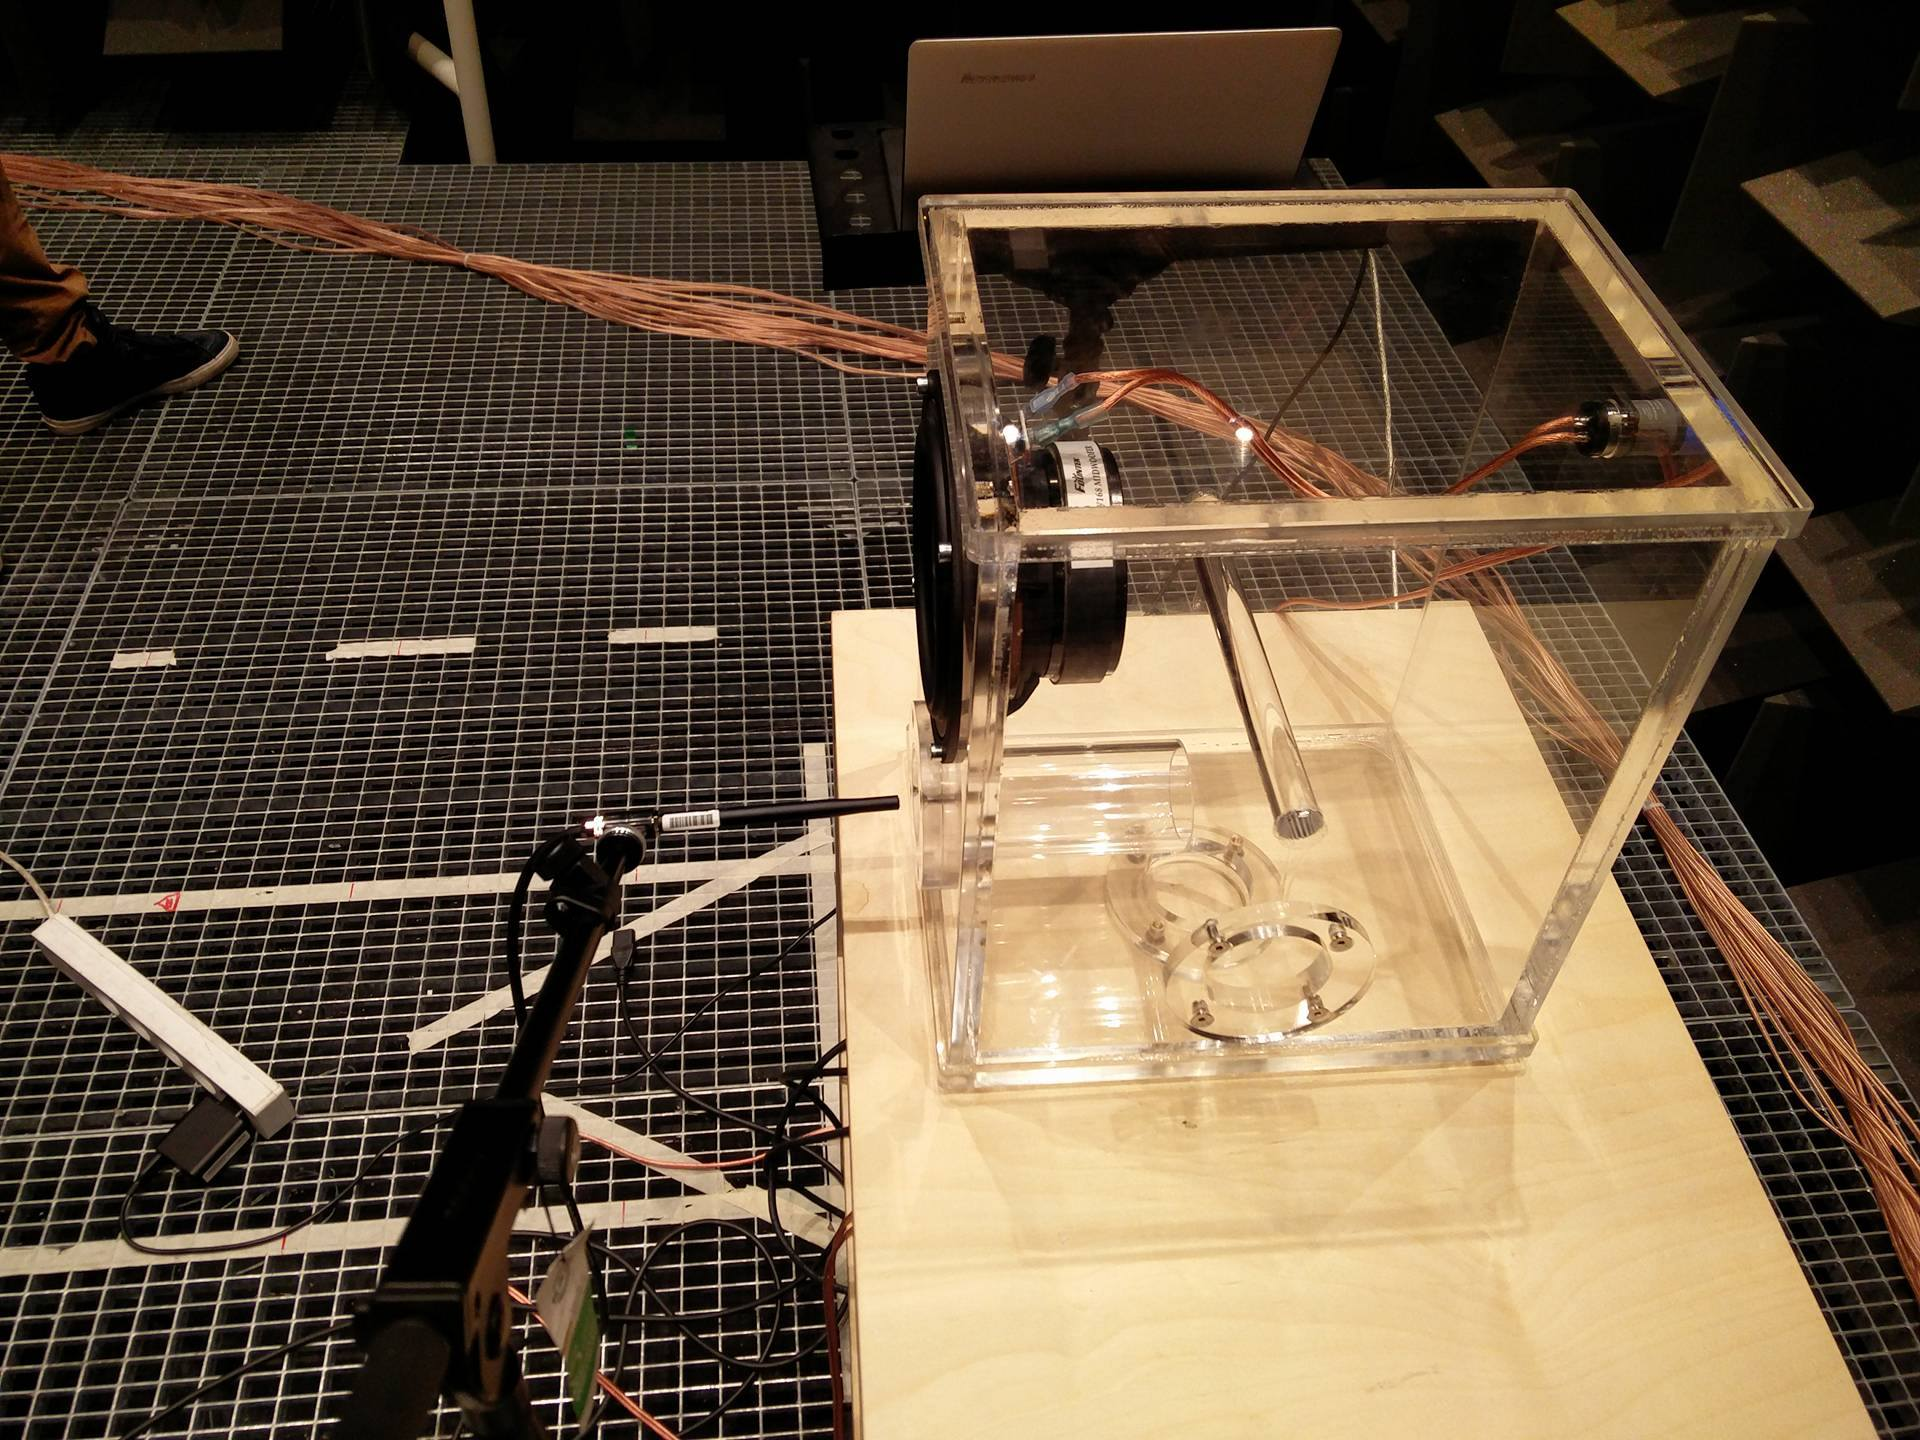
\includegraphics[width=0.5\textwidth]{Billeder/MaalBasrefleks}
	\caption{Typisk måleopstilling for måling af basrefleksens frekvenskarakteristik}
\end{figure}
\subsection{Indflydelse af basrefleksens placering}